\section{Project size estimation - Function Points}
In this section the project size will be evaluated in terms of unadjusted function points. Given the following table summarizing the complexity weights of various function types, a detailed analysis will follow in the upcoming paragraphs.\\

\begin{figure}[h!]
        \centering
        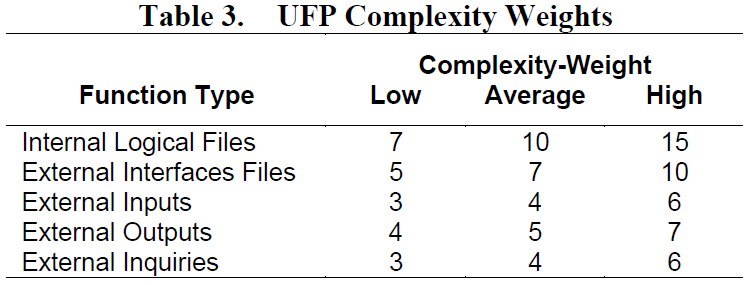
\includegraphics[width=0.7\columnwidth]{TabWeights2}
        \caption{Weights values}
        \label{fig:tw2}
\end{figure}

\subsection{INPUT}
    \paragraph {Passenger}
        \begin{itemize}
            \item \textbf{Login/Logout}: These operations con be considered with a \textit{Low} weight as they involve only one entity. 2 x 3 = \textbf{6 FPs}
            \item \textbf{Registration}: This operation involves a few more input data but still involves one entity, so it can be considered as \textit{Low} weight. 1 x 3 = \textbf{3 FPs}
            \item \textbf{Ride request / reservation}: These are quite complex, in fact they require some data from the user and the interaction with other entities. So consider these as \textit{High} weight. 2 x 6 = \textbf{12 FPs}
        \end{itemize}
    
    \paragraph{Taxi Driver}
        \begin{itemize}
            \item \textbf{Accept / Decline request}: This operation can be considered of \textit{Average} weight, as it requires only an interaction from the user, but in involves two other entities, request and passenger. 2 x 4 = \textbf{8 FPs}
            \item \textbf{Start / Stop ride}: Again this operation requires a single interaction from user, but involves other two entities, ride and Passenger. So we adopt an \textit{Average} weight. 2 x 4 = \textbf{8 FPs}
        \end{itemize}

\subsection{OUTPUT}
    \begin{itemize}
        \item \textbf{Total fare of a ride}: This operation requires information from three different entities, ride, driver and passenger, it can be considered of \textit{High} weight. 1 x 7 = \textbf{7 FPs}
        \item \textbf{Notification for accepted ride}: This operation requires information from two different entities, driver and passenger, it can be considered of \textit{Average} weight. 1 x 5 = \textbf{5 FPs}
        \item \textbf{Notification for ride request}: This operation requires information from three different entities, request, driver and passenger, it can be considered of \textit{High} weight. 1 x 7 = \textbf{7 FPs}
    \end{itemize}

\subsection{INQUIRY}
    \paragraph {Passenger}
        \begin{itemize}
            \item \textbf{Rides Log}: This operation requires data from Passenger and Rides. It is a quite easy operation so can be considered of \textit{Low} weight. 1 x 3 = \textbf{3 FPs}
        \end{itemize}
    
    \paragraph{Taxi Driver}
        \begin{itemize}
            \item \textbf{Notifications}: This operation requires data Requests and Driver entities but still remains an easy operation, so can be considered of \textit{Low} weight. 1 x 3 = \textbf{3 FPs}
            \item \textbf{Passengers on board}: This operation requires information Passengers, Rides and Driver entities so can be considered of \textit{High} weight. 1 x 6 = \textbf{6 FPs}
        \end{itemize}

\subsection{ILF}
The following entities will be used to store information needed for the application:
\textbf{Passengers}, \textbf{Taxis}, \textbf{Requests}, \textbf{Rides} and \textbf{Drivers}.
They all have a simple structure, except for the Request entity that is a little bit more complicated. So we assigned a \textit{Low} weight to all the entities, except for Request that has an \textit{Average} weight. 4 x 7 + 1 x 10 = \textbf{38 FPs}
\subsection{EIF}
    \begin{itemize}
        \item \textbf{GPS location}: This file contains the GPS coordinates of the vehicle. Can be considered with a simple structure so we assigned a \textit{Low} weight. 1 x 5 = \textbf{5 FPs}
        \item \textbf{Payment data}: This file contains data about the payment. It is quite simple so we assigned a \textit{Low} weight. 1 x 5 = \textbf{5 FPs}
        \item \textbf{Path data}: This is a complex structure acquired from the Google Maps API, we assigned an \textit{High} weight. 1 x 10 = \textbf{10 FPs}
    \end{itemize}

\subsection{Summary}
 {\renewcommand{\arraystretch}{1.5}

\begin{tabularx}{\textwidth}{X  r}
    \hline 
    \textbf{Function Type} & \textbf{Total FP}\\ 
    \hline 
    
    Input &  6 + 3 + 12 + 8 + 8 = 37 FPs\\
    \hline 
    Output & 7 + 5 + 7 = 19 FPs\\
    \hline
    Inquiry & 3 + 3 + 6 = 12 FPs\\
    \hline
    ILF & 38 FPs\\
    \hline
    EIF & 5 + 5 + 10 = 20 FPs\\
    \hline
    Total & 37 + 19 + 12 + 38 + 20 = \textbf{126 FPs}\\
    \hline
\end{tabularx}}